\chapter{Forking in a nutshell}
\label{ch:forking}

\begin{summary}
This chapter will look into the process of upgrading the network. It explains what forking the blockchain means and what are the consequences.
\end{summary}

\section{Software Development Forks}
A software project fork occurs when some developers take a copy of the project and develop it independently of the original. This is not just another development branch, this is a \keyword{divergence of direction}; effectively we now have two separate projects and the community splits accordingly.

Project forking is an important aspect of open source development allowing different opinions and roadmaps to become a reality. Some notable examples are:

\begin{itemize}
\item Linux Mint from Ubuntu (and Ubuntu from Debian)
\item MariaDB from MySQL
\item PostgreSQL fron Ingres
\item OpenSSH from OSSH
\item Inkscape from Sodipodi (and Sodipodi from Gill)
\item Plex from XBMC
\item And many many more.
\end{itemize}

\section{Blockchain Forks}
A blockchain fork occurs when different peers on the network run code that implements incompatible rules. This can happen because of a software project fork when some developers take a copy of a blockchain project and develop it independently of the original but it could also happen due to a bug in a simple upgrade.

If the implemented rules change to a degree that the messages are not compatible with the original rules then some peers will start rejecting some of the messages with the possibility that the peer to peer network is effectively split into two networks, depending on the kind of change that occurred; i.e. the blockchain will fork and different peers will add blocks to different blockchains.

Since running new code might result in a network (aka chain) fork the only way to update the Bitcoin protocol\footnote{In particular the consensus rules.} is by forking.

\begin{note}
Temporary branching on the blockchain can sometimes occur and it is part of the Nakamoto consensus. Forking refers to compatibility breaking changes between peers.
\end{note}

Forks can occur when nodes on the network run different versions of the software. This is the case when the Bitcoin software is being upgraded, e.g. from core v0.11.2 to core v0.12.0. This is a scheduled fork and if all peers agree on the change and upgrade the software in a timely manner there will be no issues.

Alternatively, competing versions might run, e.g. Bitcoin Core v0.12.0 and Bitcoin Classic v0.12.0. The two groups will have different visions on how they wish Bitcoin to evolve and thus compete to gain the majority of the hashing power in order for their chain to prevail\footnote{Prevail in terms of hashing power. Other than that both networks can co-exist.}.

We can have intentional forks due to software upgrades or alternative implementations, and unintentional forks due to incompatibilities caused by bugs.

There are two different types of blockchain forking:
\begin{description}
\item[Soft-forks:] blocks that would be valid (to old nodes) are now invalid
\item[Hard-forks:] blocks that would be invalid (to old nodes) are now valid
\end{description}


\section{Soft-forks}
Blocks that would be valid are now invalid; thus new blocks created are a subset of the possible blocks that the old rule-set would allow. Both old and new nodes will accept new blocks. However, blocks created by old nodes will be accepted only by old nodes.

In theory, even 51\% of the hashrate would be enough for the new chain since it will consistently (over a period) have the longer chain. Since the longer chain consists of new blocks which are valid by both old and new nodes, the old nodes will switch to the chain consisting new node blocks; thus the blockchain itself remains compatible between all the nodes.

Soft-forks are backward compatible; valid inputs of the new version are also valid by the old version. They do not force old nodes to upgrade or else consider them out of consensus.

A easy to understand example would be a new rule that decreases the maximum block size to 300kB. From now on new nodes will accept as valid only blocks that are 300kB or less. These blocks are also valid to the old nodes so it is a soft-fork change. Since the new blocks have the majority of the hashrate the chain will eventually consist of only 300kB blocks and old nodes will slowly upgrade to the new rules\footnote{They don't have to upgrade but their larger than 300kB blocks will never be finalized in the blockchain, so they might as well upgrade.}.

Another example is Segwit but that involved several changes. Several sophisticated modifications were required to implement it a soft-fork; see section~\ref{sec:segwit} for more details.

To summarize, in a typical soft-fork, the new rules do not clash with the old rules.
For a step by step example of a soft-fork and how new blocks are added on top see figure~\ref{fig:soft-fork-example}.

\begin{figure}[h]
\begin{center}
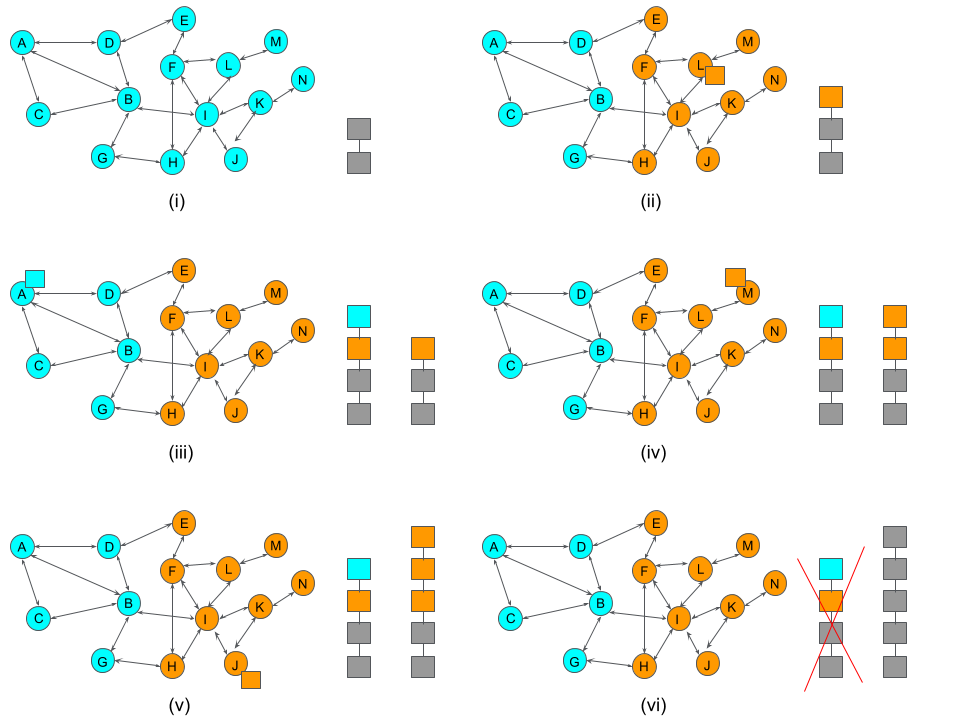
\includegraphics[scale=0.4]{images/soft-fork-example}
\caption{A soft-fork example.}
\label{fig:soft-fork-example}
\end{center}
\end{figure}

\begin{enumerate}[(i)]
\item Initially our example network has only two blocks and all nodes are in sync.
\item Then, a soft-fork upgrade occurs where 67\% of the network uses the new rules and one of the new nodes finds a new block. That block is accepted by everyone since new rules are a subset of the old rules. All the nodes are still in sync.
\item Next, a block with the old ruleset is created. It is only accepted by old nodes and thus we now have a temporary split.
\item Next another block with the new rules is found. It is accepted only by the new rules since the chains' tips are different. Note that the chains are now of equal size.
\item Then yet another block with the new rules is found (67\% chance!). Again, it is added on top of the chain with an orange block on top. However, the chain with the new rules is now the longest chain! 
\item The old nodes are forced to follow the longest chain and thus the network is in sync again.
\end{enumerate}

The actual blockchain will always sync to the longest chain and the above mentioned percentages have to do with the hashing rate and thus the miners. However, to other stakeholders like users and merchants a prolonged soft-fork could prove very disruptive.

Specifically, if a merchant is using the old chain for its transactions it is possible that their transactions are ignored when the node switches to the new nodes’ (longest) chain. In between, that would lead to fake confirmations and potential \emph{double spends}.

Typically, if hashrate is obviously leaning to one side the rest of the network nodes will follow; miners to stop losing rewards and merchants/users to have move consistent transactions.

Note that if the new nodes have 49\% or less they will not be able to sustain the longest chain and two incompatible chains will be created that cannot re-sync, leading to a \emph{temporary} hard-fork.

\begin{note}
Whenever a longer alternative chain appears nodes have to accept it and substitute their latest blocks up until a common parent is found with the new chain. When that happers we say that a re-organization or \emph{reorg} occured.
\end{note}


\section{Hard-forks}
Blocks that would be invalid are now valid; thus new blocks created are a superset of the possible blocks that the old rule-set would allow. Neither old or new nodes will accept blocks created from the others\footnote{Of course this assumes that the new incompatible feature is being used in that block.}.

Irrespective of the hashing rate this will result in a chain split that will not be able to be resolved unless one of the sides changes software.

For a step by step example of a hard-fork and how new blocks are added on top see figure~\ref{fig:hard-fork-example}.

\begin{figure}[h]
\begin{center}
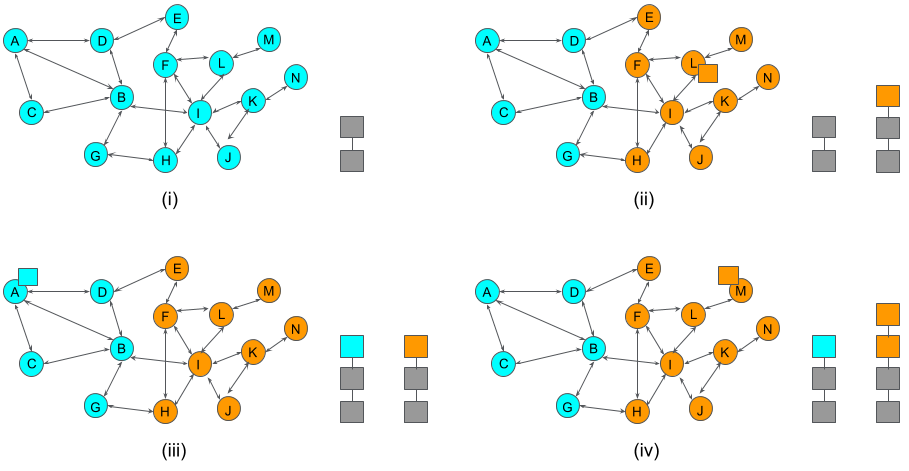
\includegraphics[scale=0.4]{images/hard-fork-example}
\caption{A hard-fork example.}
\label{fig:hard-fork-example}
\end{center}
\end{figure}

\begin{enumerate}[(i)]
\item Initially our example network has only two blocks and all nodes are in sync.
\item Then, a soft-fork upgrade occurs where 67\% of the network uses the new rules and one of the new nodes finds a new block. The new block is accepted only by the nodes with the new rules and thus we have a split.
\item Next a block is found based on the old rules which is accepted only by the nodes running the old rules.
\item Finally, another block is found by the nodes running the new rules which goes on the respective chain. The old nodes will never accept the incompatible blocks even from a longer chain. The split is permanent.
\end{enumerate}


If a hard-fork occurs the network is effectively split in two. The mining hashrate is split in two as are the merchants and users. If one side does not change their software a hard-fork can permanently split the community in two, effectively having two separate coins from that point onwards.

The same amount of bitcoins will exist in both chains and users will be able to access both. Miners, users and merchants have to choose which side to support and in some cases merchants/users can choose to support both; one of the coins will probably be termed an altcoin and supported as such.

All transactions after the split are in danger of being rolled back (e.g. allow some users to double-spend) if the fork resolves. 

A chain fork also has potential replay attacks; signed transaction in one chain to be relayed on the other chain. For example, a merchant that gets some bitcoins for a product, replays the transaction on the other chain to get the coins of the other chain as well.

\subsection*{Hard-fork first example}
In June 2010 Bitcoin core v0.2.10 introduced a change to the protocol that was not forward compatible. The version messages exchanged by nodes at connection time have changed format and included checksum values.

Since this would lead to a hard-fork ample time was given for all miners, users and merchants to upgrade before the activation of the new feature.

The new feature was activated in February 2012 and it happened without any incident.


\subsection*{Hard-fork second example}
In August 2010 an integer overflow bug was identified\footnote{https://bitcointalk.org/index.php?topic=822.0} in Bitcoin core v0.3.9 were billions of bitcoins could be erroneously sent. The community quickly coordinated and released v0.3.10 which fixed the issue by checking more thoroughly the integer limits.
% coordinated: https://bitcointalk.org/index.php?topic=823.40
% fixed: https://github.com/bitcoin/bitcoin/commit/d4c6b90ca3f9b47adb1b2724a0c3514f80635c84#diff-118fcbaaba162ba17933c7893247df3aR1013

The new version was soon run by the majority of nodes\footnote{Back then all nodes were mining nodes.} and thus the new chain overtook the old erroneous one removing the inflation bug.


\subsection*{Hard-fork third example}
In March 2013, Bitcoin core v0.8 switched its database for storing information about blocks and transactions from BerkeleyDB to LevelDB because it was more efficient. However, with the upgrade came an unexpected bug that caused incompatibility between nodes running BerkeleyDB and the new ones running LevelDB.

The bug was that BerkeleyDB had a limit on effectively how many changes it can make to the database while LevelDB did not. The limit was reached and old nodes rejected the block that caused it while new nodes accepted it; blocks that would be invalid where now valid.

The fork was detected quickly by IRC users reporting conflicting block heights on their nodes. The new chain had the majority of the hash rate and thus the old nodes were left behind with a possibility of finding and notifying them being slim.

Major miners were easier to find however and it was quickly agreed that they switch back to v0.7 so that the majority of the hashrate was that of the old nodes. This way thousands of users being on old nodes would not need to upgrade their clients and that would minimize disruption. 

Indeed, since it was communicated to most miners that a bug caused a split and, more importantly, since the majority of the hashrate was in the old chain the rest of the miners had strong incentive to revert to the old version as well to be part of the valid chain (and thus get rewards).

There was no political, economic or other incentive to continue with the new chain and thus it died away. Some miners lost their rewards and a merchant fell victim to a successful double spend but other than that the incident was painless.

\section{Upgrading Bitcoin}
During the first years of its existence upgrading Bitcoin involved notifying node owners to upgrade via forums and mailing lists. The community was smaller and more in-line regarding the future of Bitcoin.

As the network grew however coordinating via forums could not scale well so new mechanisms were added to improve the process.

New proposals came up on how miners can signal agreement for particular upgrades. If there was enough consensus the upgrade would be activated. Two such proposals were BIP-34\footnote{https://github.com/bitcoin/bips/blob/master/bip-0034.mediawiki} (now obsolete) and BIP-9\footnote{https://github.com/bitcoin/bips/blob/master/bip-0009.mediawiki} that is currently used.

\subsection*{BIP-34}
The block version was traditionally 1. The BIP suggested that when miners want to support a proposal they would increase the block version to signal that to others and specify in the coinbase input the block height when the upgrade will be activated given it has enough support. The (convention) rules were as follows:

To add a new feature a block version number (e.g. 2) would be associated with it as well as a block height for activation.

\begin{itemize}
\item If 750 out 1000 blocks\footnote{510 out of 1000 for testnet} have block version of 2 then reject invalid v2 blocks (if no block height included)
\item If 950 out of 1000 blocks\footnote{750 out of 1000 for testnet} have block version of 2 then reject all block version 1 blocks
\end{itemize}

The BIPs activated with this signaling process were, BIP-32 (v2), BIP-65 (v3) and BIP-66 (v4).


\subsection*{BIP-9}
BIP-34 allowed only one upgrade at a time and no easy way to reject a proposal to replace it with another. BIP-9 solves these issues with the following (convention) rules:

\begin{itemize}
\item The remaining 29 bits of the block version field can be used to signal for 29 proposals, potentially in parallel
\item A structure is defined with:
	\begin{itemize}
	\item name
	\item bit, the block version bit used to signal for this change
	\item starttime, time (Median Time-Past, BIP-113\footnote{https://github.com/bitcoin/bips/blob/master/bip-0113.mediawiki}) when signalling can begin
	\item timeout, time (MTP) when change is considered rejected if not activated by then
	\end{itemize}
\item Threshold for activation is 95\%
\item Signalling is based on the whole 2016 blocks of a re-target interval
\item If threshold is passed activation occurs one re-target interval later
\end{itemize}

BIP-9 was used to activate proposal ``csv'' that contained BIPs 66, 112 and 113 and proposal ``segwit'' that included BIPs 141, 143 and 147. There is a list\footnote{BIP-9 was used to activate proposal “csv” that contained BIPs 66, 112 and 113. There is a list of all BIP-9 deployments (both past and current ones).} of all BIP-9 deployments (both past and current ones).

\begin{note}
The Bitcoin community opted to do only soft-fork upgrades to minimize potential disuption to the network. To that end extra precautions and effort is required in the upgrade design and implementation. A notable example is the \emph{Segregated Witness} or \emph{segwit} upgrade. The latter would be easier to implement as a hard-fork but since those are contentious they had to come up with a design that allowed the upgrade to happen as a soft-fork. 
\end{note}

The segwit upgrade was quite contentious and there was a lot of political agendas and drama involved. A good walkthrough was published in Bitcoin Magazine\footnote{https://bitcoinmagazine.com/articles/long-road-segwit-how-bitcoins-biggest-protocol-upgrade-became-reality} and several other online resources.


